% Options for packages loaded elsewhere
\PassOptionsToPackage{unicode}{hyperref}
\PassOptionsToPackage{hyphens}{url}
\PassOptionsToPackage{dvipsnames,svgnames,x11names}{xcolor}
%
\documentclass[
  letterpaper,
]{krantz}

\usepackage{amsmath,amssymb}
\usepackage{iftex}
\ifPDFTeX
  \usepackage[T1]{fontenc}
  \usepackage[utf8]{inputenc}
  \usepackage{textcomp} % provide euro and other symbols
\else % if luatex or xetex
  \usepackage{unicode-math}
  \defaultfontfeatures{Scale=MatchLowercase}
  \defaultfontfeatures[\rmfamily]{Ligatures=TeX,Scale=1}
\fi
\usepackage{lmodern}
\ifPDFTeX\else  
    % xetex/luatex font selection
\fi
% Use upquote if available, for straight quotes in verbatim environments
\IfFileExists{upquote.sty}{\usepackage{upquote}}{}
\IfFileExists{microtype.sty}{% use microtype if available
  \usepackage[]{microtype}
  \UseMicrotypeSet[protrusion]{basicmath} % disable protrusion for tt fonts
}{}
\makeatletter
\@ifundefined{KOMAClassName}{% if non-KOMA class
  \IfFileExists{parskip.sty}{%
    \usepackage{parskip}
  }{% else
    \setlength{\parindent}{0pt}
    \setlength{\parskip}{6pt plus 2pt minus 1pt}}
}{% if KOMA class
  \KOMAoptions{parskip=half}}
\makeatother
\usepackage{xcolor}
\setlength{\emergencystretch}{3em} % prevent overfull lines
\setcounter{secnumdepth}{5}
% Make \paragraph and \subparagraph free-standing
\ifx\paragraph\undefined\else
  \let\oldparagraph\paragraph
  \renewcommand{\paragraph}[1]{\oldparagraph{#1}\mbox{}}
\fi
\ifx\subparagraph\undefined\else
  \let\oldsubparagraph\subparagraph
  \renewcommand{\subparagraph}[1]{\oldsubparagraph{#1}\mbox{}}
\fi

\usepackage{color}
\usepackage{fancyvrb}
\newcommand{\VerbBar}{|}
\newcommand{\VERB}{\Verb[commandchars=\\\{\}]}
\DefineVerbatimEnvironment{Highlighting}{Verbatim}{commandchars=\\\{\}}
% Add ',fontsize=\small' for more characters per line
\usepackage{framed}
\definecolor{shadecolor}{RGB}{241,243,245}
\newenvironment{Shaded}{\begin{snugshade}}{\end{snugshade}}
\newcommand{\AlertTok}[1]{\textcolor[rgb]{0.68,0.00,0.00}{#1}}
\newcommand{\AnnotationTok}[1]{\textcolor[rgb]{0.37,0.37,0.37}{#1}}
\newcommand{\AttributeTok}[1]{\textcolor[rgb]{0.40,0.45,0.13}{#1}}
\newcommand{\BaseNTok}[1]{\textcolor[rgb]{0.68,0.00,0.00}{#1}}
\newcommand{\BuiltInTok}[1]{\textcolor[rgb]{0.00,0.23,0.31}{#1}}
\newcommand{\CharTok}[1]{\textcolor[rgb]{0.13,0.47,0.30}{#1}}
\newcommand{\CommentTok}[1]{\textcolor[rgb]{0.37,0.37,0.37}{#1}}
\newcommand{\CommentVarTok}[1]{\textcolor[rgb]{0.37,0.37,0.37}{\textit{#1}}}
\newcommand{\ConstantTok}[1]{\textcolor[rgb]{0.56,0.35,0.01}{#1}}
\newcommand{\ControlFlowTok}[1]{\textcolor[rgb]{0.00,0.23,0.31}{#1}}
\newcommand{\DataTypeTok}[1]{\textcolor[rgb]{0.68,0.00,0.00}{#1}}
\newcommand{\DecValTok}[1]{\textcolor[rgb]{0.68,0.00,0.00}{#1}}
\newcommand{\DocumentationTok}[1]{\textcolor[rgb]{0.37,0.37,0.37}{\textit{#1}}}
\newcommand{\ErrorTok}[1]{\textcolor[rgb]{0.68,0.00,0.00}{#1}}
\newcommand{\ExtensionTok}[1]{\textcolor[rgb]{0.00,0.23,0.31}{#1}}
\newcommand{\FloatTok}[1]{\textcolor[rgb]{0.68,0.00,0.00}{#1}}
\newcommand{\FunctionTok}[1]{\textcolor[rgb]{0.28,0.35,0.67}{#1}}
\newcommand{\ImportTok}[1]{\textcolor[rgb]{0.00,0.46,0.62}{#1}}
\newcommand{\InformationTok}[1]{\textcolor[rgb]{0.37,0.37,0.37}{#1}}
\newcommand{\KeywordTok}[1]{\textcolor[rgb]{0.00,0.23,0.31}{#1}}
\newcommand{\NormalTok}[1]{\textcolor[rgb]{0.00,0.23,0.31}{#1}}
\newcommand{\OperatorTok}[1]{\textcolor[rgb]{0.37,0.37,0.37}{#1}}
\newcommand{\OtherTok}[1]{\textcolor[rgb]{0.00,0.23,0.31}{#1}}
\newcommand{\PreprocessorTok}[1]{\textcolor[rgb]{0.68,0.00,0.00}{#1}}
\newcommand{\RegionMarkerTok}[1]{\textcolor[rgb]{0.00,0.23,0.31}{#1}}
\newcommand{\SpecialCharTok}[1]{\textcolor[rgb]{0.37,0.37,0.37}{#1}}
\newcommand{\SpecialStringTok}[1]{\textcolor[rgb]{0.13,0.47,0.30}{#1}}
\newcommand{\StringTok}[1]{\textcolor[rgb]{0.13,0.47,0.30}{#1}}
\newcommand{\VariableTok}[1]{\textcolor[rgb]{0.07,0.07,0.07}{#1}}
\newcommand{\VerbatimStringTok}[1]{\textcolor[rgb]{0.13,0.47,0.30}{#1}}
\newcommand{\WarningTok}[1]{\textcolor[rgb]{0.37,0.37,0.37}{\textit{#1}}}

\providecommand{\tightlist}{%
  \setlength{\itemsep}{0pt}\setlength{\parskip}{0pt}}\usepackage{longtable,booktabs,array}
\usepackage{calc} % for calculating minipage widths
% Correct order of tables after \paragraph or \subparagraph
\usepackage{etoolbox}
\makeatletter
\patchcmd\longtable{\par}{\if@noskipsec\mbox{}\fi\par}{}{}
\makeatother
% Allow footnotes in longtable head/foot
\IfFileExists{footnotehyper.sty}{\usepackage{footnotehyper}}{\usepackage{footnote}}
\makesavenoteenv{longtable}
\usepackage{graphicx}
\makeatletter
\def\maxwidth{\ifdim\Gin@nat@width>\linewidth\linewidth\else\Gin@nat@width\fi}
\def\maxheight{\ifdim\Gin@nat@height>\textheight\textheight\else\Gin@nat@height\fi}
\makeatother
% Scale images if necessary, so that they will not overflow the page
% margins by default, and it is still possible to overwrite the defaults
% using explicit options in \includegraphics[width, height, ...]{}
\setkeys{Gin}{width=\maxwidth,height=\maxheight,keepaspectratio}
% Set default figure placement to htbp
\makeatletter
\def\fps@figure{htbp}
\makeatother
\newlength{\cslhangindent}
\setlength{\cslhangindent}{1.5em}
\newlength{\csllabelwidth}
\setlength{\csllabelwidth}{3em}
\newlength{\cslentryspacingunit} % times entry-spacing
\setlength{\cslentryspacingunit}{\parskip}
\newenvironment{CSLReferences}[2] % #1 hanging-ident, #2 entry spacing
 {% don't indent paragraphs
  \setlength{\parindent}{0pt}
  % turn on hanging indent if param 1 is 1
  \ifodd #1
  \let\oldpar\par
  \def\par{\hangindent=\cslhangindent\oldpar}
  \fi
  % set entry spacing
  \setlength{\parskip}{#2\cslentryspacingunit}
 }%
 {}
\usepackage{calc}
\newcommand{\CSLBlock}[1]{#1\hfill\break}
\newcommand{\CSLLeftMargin}[1]{\parbox[t]{\csllabelwidth}{#1}}
\newcommand{\CSLRightInline}[1]{\parbox[t]{\linewidth - \csllabelwidth}{#1}\break}
\newcommand{\CSLIndent}[1]{\hspace{\cslhangindent}#1}

\usepackage{booktabs}
\usepackage{longtable}
\usepackage[bf,singlelinecheck=off]{caption}
\usepackage[scale=.8]{sourcecodepro}
\usepackage{hyperref}

\usepackage{framed,color}
\definecolor{shadecolor}{RGB}{248,248,248}

\renewcommand{\textfraction}{0.05}
\renewcommand{\topfraction}{0.8}
\renewcommand{\bottomfraction}{0.8}
\renewcommand{\floatpagefraction}{0.75}

\renewenvironment{quote}{\begin{VF}}{\end{VF}}
\let\oldhref\href
\renewcommand{\href}[2]{#2\footnote{\url{#1}}}

\makeatletter
\newenvironment{kframe}{%
\medskip{}
\setlength{\fboxsep}{.8em}
 \def\at@end@of@kframe{}%
 \ifinner\ifhmode%
  \def\at@end@of@kframe{\end{minipage}}%
  \begin{minipage}{\columnwidth}%
 \fi\fi%
 \def\FrameCommand##1{\hskip\@totalleftmargin \hskip-\fboxsep
 \colorbox{shadecolor}{##1}\hskip-\fboxsep
     % There is no \\@totalrightmargin, so:
     \hskip-\linewidth \hskip-\@totalleftmargin \hskip\columnwidth}%
 \MakeFramed {\advance\hsize-\width
   \@totalleftmargin\z@ \linewidth\hsize
   \@setminipage}}%
 {\par\unskip\endMakeFramed%
 \at@end@of@kframe}
\makeatother

\renewenvironment{Shaded}{\begin{kframe}}{\end{kframe}}

\usepackage{makeidx}
\makeindex

\urlstyle{tt}

\usepackage{amsthm}
\makeatletter
\def\thm@space@setup{%
  \thm@preskip=8pt plus 2pt minus 4pt
  \thm@postskip=\thm@preskip
}
\makeatother

\frontmatter
\makeatletter
\makeatother
\makeatletter
\@ifpackageloaded{bookmark}{}{\usepackage{bookmark}}
\makeatother
\makeatletter
\@ifpackageloaded{caption}{}{\usepackage{caption}}
\AtBeginDocument{%
\ifdefined\contentsname
  \renewcommand*\contentsname{Table of contents}
\else
  \newcommand\contentsname{Table of contents}
\fi
\ifdefined\listfigurename
  \renewcommand*\listfigurename{List of Figures}
\else
  \newcommand\listfigurename{List of Figures}
\fi
\ifdefined\listtablename
  \renewcommand*\listtablename{List of Tables}
\else
  \newcommand\listtablename{List of Tables}
\fi
\ifdefined\figurename
  \renewcommand*\figurename{Figure}
\else
  \newcommand\figurename{Figure}
\fi
\ifdefined\tablename
  \renewcommand*\tablename{Table}
\else
  \newcommand\tablename{Table}
\fi
}
\@ifpackageloaded{float}{}{\usepackage{float}}
\floatstyle{ruled}
\@ifundefined{c@chapter}{\newfloat{codelisting}{h}{lop}}{\newfloat{codelisting}{h}{lop}[chapter]}
\floatname{codelisting}{Listing}
\newcommand*\listoflistings{\listof{codelisting}{List of Listings}}
\makeatother
\makeatletter
\@ifpackageloaded{caption}{}{\usepackage{caption}}
\@ifpackageloaded{subcaption}{}{\usepackage{subcaption}}
\makeatother
\makeatletter
\@ifpackageloaded{tcolorbox}{}{\usepackage[skins,breakable]{tcolorbox}}
\makeatother
\makeatletter
\@ifundefined{shadecolor}{\definecolor{shadecolor}{rgb}{.97, .97, .97}}
\makeatother
\makeatletter
\makeatother
\makeatletter
\makeatother
\ifLuaTeX
  \usepackage{selnolig}  % disable illegal ligatures
\fi
\IfFileExists{bookmark.sty}{\usepackage{bookmark}}{\usepackage{hyperref}}
\IfFileExists{xurl.sty}{\usepackage{xurl}}{} % add URL line breaks if available
\urlstyle{same} % disable monospaced font for URLs
\hypersetup{
  pdftitle={Quarto CRC Book},
  pdfauthor={Jane Doe and Max Power},
  colorlinks=true,
  linkcolor={blue},
  filecolor={Maroon},
  citecolor={Blue},
  urlcolor={Blue},
  pdfcreator={LaTeX via pandoc}}

\title{Quarto CRC Book}
\author{Jane Doe and Max Power}
\date{2022-11-22}

\begin{document}
\maketitle
% you may need to leave a few empty pages before the dedication page

%\cleardoublepage\newpage\thispagestyle{empty}\null
%\cleardoublepage\newpage\thispagestyle{empty}\null
%\cleardoublepage\newpage
\thispagestyle{empty}

\begin{center}
To blah, blah, and blah.
%\includegraphics{images/dedication.pdf}
\end{center}

\setlength{\abovedisplayskip}{-5pt}
\setlength{\abovedisplayshortskip}{-5pt}

\ifdefined\Shaded\renewenvironment{Shaded}{\begin{tcolorbox}[sharp corners, enhanced, interior hidden, borderline west={3pt}{0pt}{shadecolor}, breakable, frame hidden, boxrule=0pt]}{\end{tcolorbox}}\fi

\renewcommand*\contentsname{Table of contents}
{
\hypersetup{linkcolor=}
\setcounter{tocdepth}{2}
\tableofcontents
}
\bookmarksetup{startatroot}

\hypertarget{preface}{%
\chapter*{Preface}\label{preface}}
\addcontentsline{toc}{chapter}{Preface}

\markboth{Preface}{Preface}

This is a Quarto book.

\hypertarget{software-conventions}{%
\section*{Software conventions}\label{software-conventions}}
\addcontentsline{toc}{section}{Software conventions}

\markright{Software conventions}

\begin{Shaded}
\begin{Highlighting}[]
\DecValTok{1} \OperatorTok{+} \DecValTok{1}
\end{Highlighting}
\end{Shaded}

\begin{verbatim}
2
\end{verbatim}

To learn more about Quarto books visit
\url{https://quarto.org/docs/books}.

\mainmatter

\bookmarksetup{startatroot}

\hypertarget{closeness-centrality}{%
\chapter{Closeness Centrality}\label{closeness-centrality}}

\begin{Shaded}
\begin{Highlighting}[]
\OperatorTok{!}\NormalTok{pip install networkx}
\end{Highlighting}
\end{Shaded}

\begin{verbatim}
Requirement already satisfied: networkx in /usr/local/lib/python3.10/dist-packages (3.2)
\end{verbatim}

\begin{Shaded}
\begin{Highlighting}[]
\ImportTok{import}\NormalTok{ pandas }\ImportTok{as}\NormalTok{ pd}
\ImportTok{import}\NormalTok{ numpy }\ImportTok{as}\NormalTok{ np}
\ImportTok{from}\NormalTok{ nltk.corpus }\ImportTok{import}\NormalTok{ stopwords}
\ImportTok{import}\NormalTok{ re}
\ImportTok{import}\NormalTok{ nltk}
\NormalTok{nltk.download(}\StringTok{\textquotesingle{}stopwords\textquotesingle{}}\NormalTok{)}
\NormalTok{nltk.download(}\StringTok{\textquotesingle{}wordnet\textquotesingle{}}\NormalTok{)}
\NormalTok{nltk.download(}\StringTok{\textquotesingle{}punkt\textquotesingle{}}\NormalTok{)}
\CommentTok{\# from Sastrawi.Stemmer.StemmerFactory import StemmerFactory}
\ImportTok{from}\NormalTok{ nltk.tokenize }\ImportTok{import}\NormalTok{ sent\_tokenize, word\_tokenize}
\ImportTok{from}\NormalTok{ nltk.corpus }\ImportTok{import}\NormalTok{ stopwords}
\ImportTok{from}\NormalTok{ sklearn.feature\_extraction.text }\ImportTok{import}\NormalTok{ TfidfVectorizer}
\ImportTok{from}\NormalTok{ sklearn.metrics.pairwise }\ImportTok{import}\NormalTok{ cosine\_similarity}
\ImportTok{import}\NormalTok{ networkx }\ImportTok{as}\NormalTok{ nx}
\end{Highlighting}
\end{Shaded}

\begin{verbatim}
[nltk_data] Downloading package stopwords to /root/nltk_data...
[nltk_data]   Unzipping corpora/stopwords.zip.
[nltk_data] Downloading package wordnet to /root/nltk_data...
[nltk_data] Downloading package punkt to /root/nltk_data...
[nltk_data]   Unzipping tokenizers/punkt.zip.
\end{verbatim}

\begin{Shaded}
\begin{Highlighting}[]
\NormalTok{data }\OperatorTok{=}\NormalTok{ pd.read\_csv(}\StringTok{\textquotesingle{}/content/drive/MyDrive/ppw/ppw/crawling\_berita\_new.csv\textquotesingle{}}\NormalTok{)}
\NormalTok{data}
\end{Highlighting}
\end{Shaded}

\begin{longtable}[]{@{}llll@{}}
\toprule\noalign{}
& Judul & Isi & Kategori \\
\midrule\noalign{}
\endhead
\bottomrule\noalign{}
\endlastfoot
0 & Debut IMAG Sukses, KONI Pusat: Tahun Depan Leb... & Pekan Olahraga
Bela Diri Nasional atau Indones... & Sport \\
1 & Nikmati Pengalaman Santap Steak Lezat di Mad C... & Suasana yang
nyaman dengan makanan lezat, inil... & Food \\
2 & Arus Barang Impor Jadi Diperketat, Masa Transi... & Pemerintah terus
melakukan sejumlah upaya untu... & Finance \\
3 & Jorge Martin Promosi ke Ducati di 2024? & Rider Pramac Jorge Martin
muncul sebagai penan... & Sport \\
4 & Water Purifier Tenaga Surya Menangkan AHM Best... & Jakarta - PT
Astra Honda Motor menggelar AHM B... & Edukasi \\
... & ... & ... & ... \\
155 & Sempat Mangkrak, Proyek Tol Gilimanuk-Mengwi B... & Pemerintah
akan segera melelang ulang proyek T... & Finance \\
156 & Pahami Perbedaan Tekstil, Garmen, dan Konveksi & Bisnis pakaian
adalah salah satu bisnis yang s... & Finance \\
157 & Gado-gado Racikan Mak Gobang yang Terkenal di BSD & Jakarta - Gado
Gado Mak Gobang yang dulunya be... & Food \\
158 & Harta Karun Migas Papua Sudah Dilelang, Diinca... & Kementerian
Energi dan Sumber Daya Mineral (ES... & Finance \\
159 & Megawati Hangestri: Si Pevoli Viral Indonesia ... & Megawati
Hangestri Pertiwi terus menjadi perbi... & Sport \\
\end{longtable}

\begin{Shaded}
\begin{Highlighting}[]
\NormalTok{hasil\_kalimat}\OperatorTok{=}\NormalTok{[]}
\ControlFlowTok{for}\NormalTok{ i }\KeywordTok{in} \BuiltInTok{range}\NormalTok{(}\BuiltInTok{len}\NormalTok{(data)):}
\NormalTok{  token }\OperatorTok{=}\NormalTok{ sent\_tokenize(data[}\StringTok{\textquotesingle{}Isi\textquotesingle{}}\NormalTok{][i])}
\NormalTok{  hasil\_kalimat.append(token)}
\end{Highlighting}
\end{Shaded}

\begin{Shaded}
\begin{Highlighting}[]
\NormalTok{kalimat }\OperatorTok{=}\NormalTok{ []}
\ControlFlowTok{for}\NormalTok{ i }\KeywordTok{in} \BuiltInTok{range}\NormalTok{(}\BuiltInTok{len}\NormalTok{(hasil\_kalimat)):}
  \ControlFlowTok{for}\NormalTok{ x }\KeywordTok{in} \BuiltInTok{range}\NormalTok{ (}\BuiltInTok{len}\NormalTok{(hasil\_kalimat[i])):}
\NormalTok{    datacek }\OperatorTok{=}\NormalTok{ []}
\NormalTok{    datacek.append(i)}
\NormalTok{    datacek.append(hasil\_kalimat[i][x])}
\NormalTok{    kalimat.append(datacek)}
\end{Highlighting}
\end{Shaded}

\begin{Shaded}
\begin{Highlighting}[]
\NormalTok{databaru }\OperatorTok{=}\NormalTok{ pd.DataFrame(kalimat, columns}\OperatorTok{=}\NormalTok{[}\StringTok{"Dokumen ke"}\NormalTok{, }\StringTok{"Kalimat"}\NormalTok{])}
\NormalTok{databaru}
\end{Highlighting}
\end{Shaded}

\begin{longtable}[]{@{}lll@{}}
\toprule\noalign{}
& Dokumen ke & Kalimat \\
\midrule\noalign{}
\endhead
\bottomrule\noalign{}
\endlastfoot
0 & 0 & Pekan Olahraga Bela Diri Nasional atau Indones... \\
1 & 0 & KONI Pusat menjanjikan tahun depan lebih menarik. \\
2 & 0 & IMAG pertama diselenggarakan di Kota Bekasi da... \\
3 & 0 & Ajang ini mempertandingkan 9 cabang olahraga b... \\
4 & 0 & Hasilnya, kontingen Jawa Barat menjadi juara u... \\
... & ... & ... \\
3459 & 159 & Megawati berhasil mengumpulkan 95 poin, jumlah... \\
3460 & 159 & Bahkan, ia menjadi pencetak poin terbanyak yai... \\
3461 & 159 & Adapun Red Sparks telah memenangkan tiga dari ... \\
3462 & 159 & Red Sparks dijadwalkan akan bertanding kembali... \\
3463 & 159 & Megawati dkk akan menghadapi Gimcheon Korea Ex... \\
\end{longtable}

\begin{Shaded}
\begin{Highlighting}[]
\CommentTok{\# Menghitung TF{-}IDF}
\NormalTok{vectorizer }\OperatorTok{=}\NormalTok{ TfidfVectorizer()}
\NormalTok{tfidf\_matrix }\OperatorTok{=}\NormalTok{ vectorizer.fit\_transform(databaru[}\StringTok{\textquotesingle{}Kalimat\textquotesingle{}}\NormalTok{])}
\end{Highlighting}
\end{Shaded}

\begin{Shaded}
\begin{Highlighting}[]
\CommentTok{\# Menghitung cosine similarity}
\NormalTok{cosine\_similarities }\OperatorTok{=}\NormalTok{ cosine\_similarity(tfidf\_matrix, tfidf\_matrix)}
\end{Highlighting}
\end{Shaded}

\begin{Shaded}
\begin{Highlighting}[]
\CommentTok{\# Membuat graf untuk closeness centrality}
\NormalTok{G }\OperatorTok{=}\NormalTok{ nx.from\_numpy\_array(cosine\_similarities)}

\CommentTok{\# Menghitung closeness centrality}
\NormalTok{closeness\_centrality }\OperatorTok{=}\NormalTok{ nx.closeness\_centrality(G)}

\CommentTok{\# Menambahkan closeness centrality ke dalam dataframe kalimat}
\NormalTok{databaru[}\StringTok{\textquotesingle{}Closeness Centrality\textquotesingle{}}\NormalTok{] }\OperatorTok{=}\NormalTok{ [closeness\_centrality[i] }\ControlFlowTok{for}\NormalTok{ i }\KeywordTok{in} \BuiltInTok{range}\NormalTok{(}\BuiltInTok{len}\NormalTok{(databaru))]}

\CommentTok{\# Menampilkan dataframe kalimat}
\BuiltInTok{print}\NormalTok{(databaru)}
\end{Highlighting}
\end{Shaded}

\begin{verbatim}
      Dokumen ke                                            Kalimat  \
0              0  Pekan Olahraga Bela Diri Nasional atau Indones...   
1              0  KONI Pusat menjanjikan tahun depan lebih menarik.   
2              0  IMAG pertama diselenggarakan di Kota Bekasi da...   
3              0  Ajang ini mempertandingkan 9 cabang olahraga b...   
4              0  Hasilnya, kontingen Jawa Barat menjadi juara u...   
...          ...                                                ...   
3459         159  Megawati berhasil mengumpulkan 95 poin, jumlah...   
3460         159  Bahkan, ia menjadi pencetak poin terbanyak yai...   
3461         159  Adapun Red Sparks telah memenangkan tiga dari ...   
3462         159  Red Sparks dijadwalkan akan bertanding kembali...   
3463         159  Megawati dkk akan menghadapi Gimcheon Korea Ex...   

      Closeness Centrality  
0                 0.542064  
1                 0.514661  
2                 0.649923  
3                 0.556842  
4                 0.547535  
...                    ...  
3459              0.492301  
3460              0.711714  
3461              0.681515  
3462              0.539237  
3463              0.581197  

[3464 rows x 3 columns]
\end{verbatim}

\begin{Shaded}
\begin{Highlighting}[]
\NormalTok{databaru}
\end{Highlighting}
\end{Shaded}

\begin{longtable}[]{@{}llll@{}}
\toprule\noalign{}
& Dokumen ke & Kalimat & Closeness Centrality \\
\midrule\noalign{}
\endhead
\bottomrule\noalign{}
\endlastfoot
0 & 0 & Pekan Olahraga Bela Diri Nasional atau Indones... & 0.542064 \\
1 & 0 & KONI Pusat menjanjikan tahun depan lebih menarik. & 0.514661 \\
2 & 0 & IMAG pertama diselenggarakan di Kota Bekasi da... & 0.649923 \\
3 & 0 & Ajang ini mempertandingkan 9 cabang olahraga b... & 0.556842 \\
4 & 0 & Hasilnya, kontingen Jawa Barat menjadi juara u... & 0.547535 \\
... & ... & ... & ... \\
3459 & 159 & Megawati berhasil mengumpulkan 95 poin, jumlah... &
0.492301 \\
3460 & 159 & Bahkan, ia menjadi pencetak poin terbanyak yai... &
0.711714 \\
3461 & 159 & Adapun Red Sparks telah memenangkan tiga dari ... &
0.681515 \\
3462 & 159 & Red Sparks dijadwalkan akan bertanding kembali... &
0.539237 \\
3463 & 159 & Megawati dkk akan menghadapi Gimcheon Korea Ex... &
0.581197 \\
\end{longtable}

\begin{Shaded}
\begin{Highlighting}[]
\NormalTok{databaru.to\_csv(}\StringTok{\textquotesingle{}/content/drive/MyDrive/ppw/ppw/closeness\_centrality.csv\textquotesingle{}}\NormalTok{, index}\OperatorTok{=}\VariableTok{False}\NormalTok{)}
\end{Highlighting}
\end{Shaded}

\begin{Shaded}
\begin{Highlighting}[]
\NormalTok{nx.draw(G, with\_labels}\OperatorTok{=}\VariableTok{True}\NormalTok{)}
\end{Highlighting}
\end{Shaded}

\begin{figure}[H]

{\centering 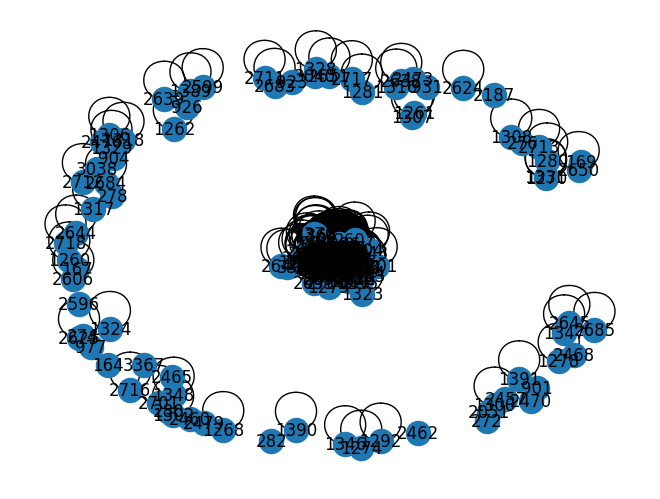
\includegraphics{Test_files/figure-pdf/cell-13-output-1.png}

}

\end{figure}

\bookmarksetup{startatroot}

\hypertarget{summary}{%
\chapter{Summary}\label{summary}}

In summary, this book has no content whatsoever.

\bookmarksetup{startatroot}

\hypertarget{references}{%
\chapter*{References}\label{references}}
\addcontentsline{toc}{chapter}{References}

\markboth{References}{References}

\hypertarget{refs}{}
\begin{CSLReferences}{0}{0}
\end{CSLReferences}



\backmatter
\printindex

\end{document}
